\newpage
\section{Neuronale Netze}
Ein neuronales Netz ist ein Zusammenschluss aus mehreren Perceptronen in verschiedenen Layern. Als Beispiel sei an
dieser Stelle die Abbildung \ref{fig:07_neuronal_network} gegeben. Diese wird ebenso verwendet, um die Ableitungskette
für ein Gewicht in diesem Fall zu zeigen. Anzumerken sei hier, dass die Kombination der gewichteten Summen mit der
Aktivierungsfunktion ein Neuron darstellt.
\begin{figure}[h!]
    \begin{center}
        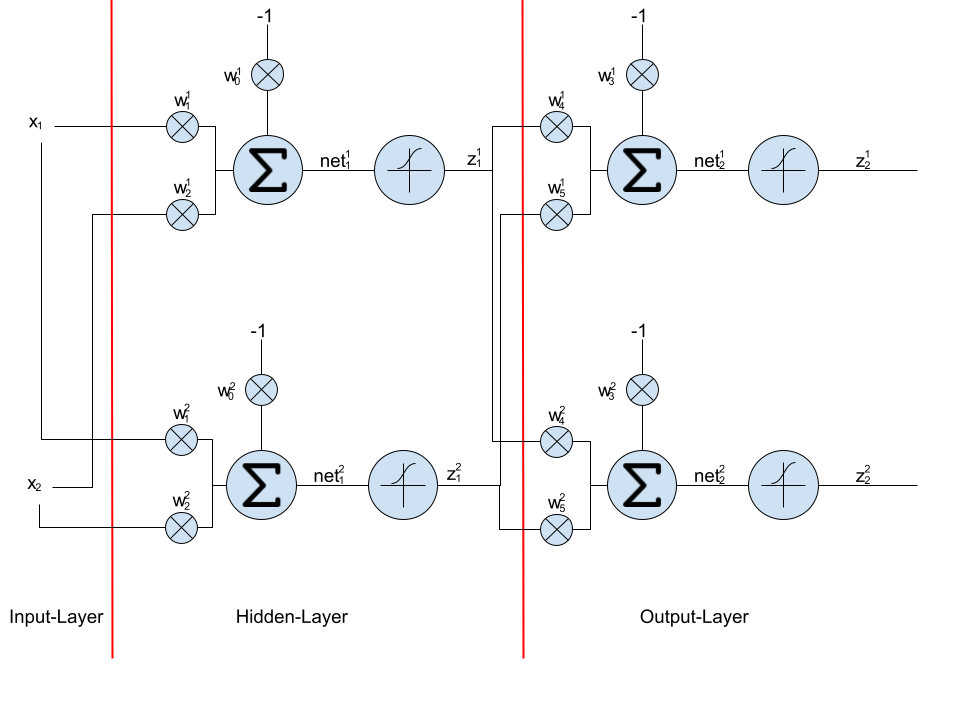
\includegraphics[width=1\linewidth]{../common/01_neuronal_network/00_resources/02_neuronales_netz.png}
    \end{center}
    \caption{Ein neuronales Netz mit einem Hidden-Layer}
    \label{fig:07_neuronal_network}
\end{figure}

\newpage
\subsection{Lernverfahren mit Gradientenabstieg}
Wie beim Perceptron auch soll nun an dieser Stelle die Komponente des Gradienten für das Gewicht $w_1^1$ gezeigt
werden. Für dieses Beispiel wird die Abbildung \ref{fig:08_neuronal_network} hinzugezogen.
\begin{figure}[h!]
    \begin{center}
        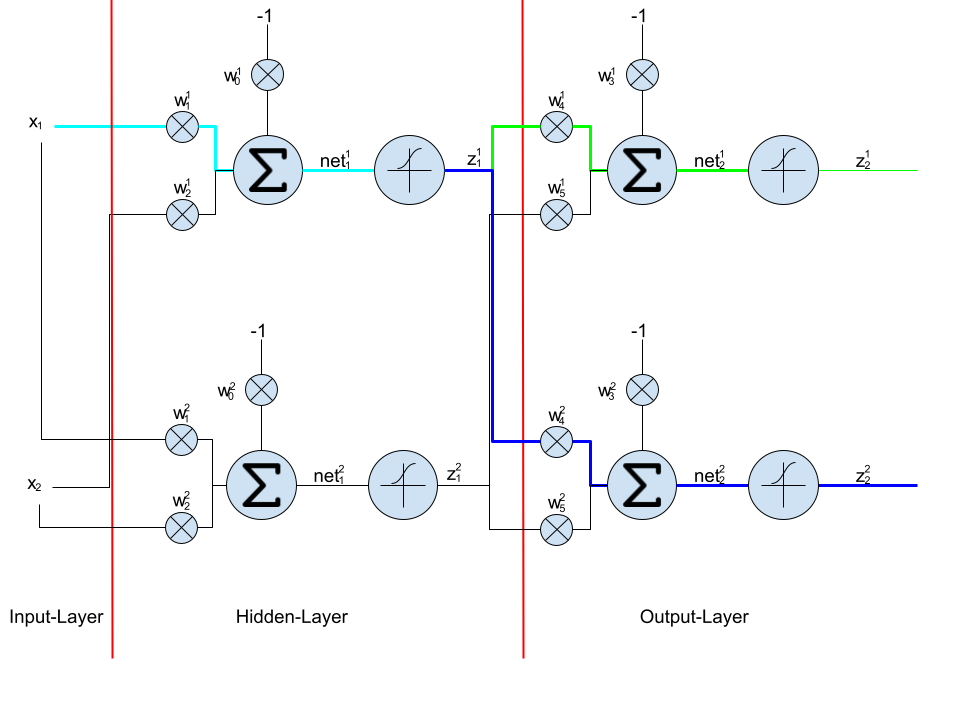
\includegraphics[width=1\linewidth]{../common/01_neuronal_network/00_resources/03_neuronales_netz_pfad.png}
    \end{center}
    \caption{Der Pfad zum Gewicht $w_1^1$ im neuronalen Netz}
    \label{fig:08_neuronal_network}
\end{figure}
Die Fehlerfunktion ist wie beim Perceptron dieselbe $P_{err} = - \frac{1}{2} \cdot \sum_i^2 (d^i - z_2^i)^2$.
In diesem Fall steht die Komponente $i$ für den Index und die $2$ für den Layer.
Zur Abbildung \ref{fig:08_neuronal_network} ist wichtig zu erkennen, dass für die Korrektor des Gewichts $w_1^1$
mehrere Wege relevant sind. Es kann einmal der grüne sowie der blaue Weg verfolgt werden. Der Teil, welcher bei
beiden gleich ist, wird cyan markiert.
Weiterhin sind folgende Werte sind bekannt:
\begin{align}
    P_{err} = - \frac{1}{2} \cdot \sum_i^2 (d^i - z_2^i)^2\\
    net_1^1 = x_1 \cdot w_1^1 + x_2 \cdot w_2^1 - w_0^1\\
    z_1^1 = \frac{1}{1 + e^{-net_1^1}}\\
    net_1^2 = x_1 \cdot w_1^2 + x_2 \cdot w_2^2 - w_0^2\\
    z_1^2 = \frac{1}{1 + e^{-net_1^2}}\\
    net_2^1 = z_1^1 \cdot w_4^1 + z_1^2 \cdot w_5^1 - w_3^1\\
    z_2^1 = \frac{1}{1 + e^{-net_2^1}}\\
    net_2^2 = z_1^1 \cdot w_4^2 + z_1^2 \cdot w_5^2 - w_3^2\\
    z_2^2 = \frac{1}{1 + e^{-net_2^2}}
\end{align}
Der Gradient für die Gewichte setzt sich wie nachfolgend zusammen:
\begin{align}
    \vec{\nabla} = (w_0^1, w_1^1, w_2^1, w_0^2, w_1^2, w_2^2, w_3^1, w_4^1, w_5^1, w_3^2, w_4^2, w_5^2)
\end{align}
Die Korrektur in einem Schritt kann wiederum über den Vektor der Gewichte $\vec{w}$ erfolgen.
\begin{align}
    \vec{w}_{neu} = \vec{w}_{alt} + \lambda \cdot \vec{\nabla}
\end{align}
Wie bereits erwähnt wird nur die Komponente $w_1^1$ aus dem Vektor $\vec{\nabla}$
berücksichtigt. Um diesen herzuleiten, müssen alle Pfade zum Gewicht berücksichtigt werden.
In dem Fall gibt es, wie in Abbildung \ref{fig:08_neuronal_network} entnommen werden kann, deren zwei.
Die Funktionskette ist in Gleichung \ref{eq:03_funktions_kette} ersichtlich. Es werden nur die wirklich relevanten Aufrufe
gezeigt.
\begin{multline}
    P_{err} = - \frac{1}{2} \cdot (d^1 - z_2^1(net_2^1(w_4^1 \cdot z_1^1(net_1^1(w_1^1 \cdot x_1, w_2^1 \cdot x_2, -w_0^1)), z_1^2 \cdot w_5^1, -w_3^1)))^2 +\\\label{eq:03_funktions_kette}
    - \frac{1}{2} \cdot (d^2 - z_2^2(net_2^2(w_4^2 \cdot z_1^1(net_1^1(w_1^1 \cdot x_1, w_2^1 \cdot x_2, -w_0^1)), z_1^2 \cdot w_5^2, -w_3^2)))^2
\end{multline}
Dementsprechend werden die beiden Pfade für die Komponente des Gradienten für $w_1^1$ berücksichtigt.
\begin{multline}
    \frac{\delta P_{err}}{\delta w_1^1} = \frac{\delta P_{err}}{\delta z_2^1(w_1^1)} \cdot \frac{\delta z_2^1(w_1^1)}{\delta net_2^1(w_1^1)} \cdot \frac{\delta net_2^1(w_1^1)}{\delta z_1^1(w_1^1)} \cdot \frac{\delta z_1^1{w_1^1}}{\delta net_1^1(w_1^1)} \cdot \frac{\delta net_1^1(w_1^1)}{\delta w_1^1} +\\
    \frac{\delta P_{err}}{\delta z_2^2(w_1^1)} \cdot \frac{\delta z_2^2(w_1^1)}{\delta net_2^2(w_1^1)} \cdot \frac{\delta net_2^2(w_1^1)}{\delta z_1^1(w_1^1)} \cdot \frac{\delta z_1^1{w_1^1}}{\delta net_1^1(w_1^1)} \cdot \frac{\delta net_1^1(w_1^1)}{\delta w_1^1}
\end{multline}
Anders ausgedrückt lautet demnach die Komponente:
\begin{multline}
    w_{1,korr}^1 = (d^1 - z_2^1) \cdot z_2^1(1 - z_2^1) \cdot w_4^1 \cdot z_1^1(1 - z_1^1) \cdot x_1 +\\
    (d^2 - z_2^2) \cdot z_2^2(1 - z_2^2) \cdot w_4^2 \cdot z_1^1(1 - z_1^1) \cdot x_1
\end{multline}
An dieser Stelle sei angemerkt, dass dieses Verfahren durchaus funktioniert, jedoch wachsen die Ableitungsterme
exponentiell mit der Anzahl Neuronen in den Layern. Aus diesem Grund ist der Gradientenabstieg so nicht brauchbar in
der Praxis. Was jedoch auffällt ist die Tatsache, dass einmal berechnete Ableitungsketten wiederverwendet werden können.
Gedanklich kann an dieser Stelle z.B. die Ableitungskette für $w_2^1$ hinzugezogen werden. Man erkennt relativ schnell,
dass viele Berechnung, welche schon für $w_1^1$ gemacht wurden, wiederauftreten. Auf Grundlage dieser Idee der
dynamischen Programmierung wurde der Backpropagation Algorithmus entwickelt.

\newpage
\subsection{Lernverfahren mit Backpropagation}
Der grosse Vorteil dieses Verfahrens ist die Berechnungszeit, welche im Vergleich zum reinen Gradientenabstieg nur noch
linear mit den Anzahl der Gewichte wächst. So werden einmal berechnete Ableitungsketten gespeichert und wiederverwendet.
Der Input-Layer wird nicht beachtet, dieser ist für die Berechnung irrelevant. Die verbleibenden Layer (Hidden-, Output-Layer)
bilden die zwei zu unterscheidenden Fälle des Algorithmus.
\\

Zuerst betrachtet man den Fall, wo es sich um den Output-Layer handelt. Um dies zu veranschaulichen, kann
die Abbildung \ref{fig:08_backpropagation_output} betrachtet werden. Auf der rechten Seite der Abbildung sind die Werte ersichtlich,
die zu diesem Zeitpunkt bekannt sind. In dem Fall gibt es keine folgende Schicht, da es sich selbst um den Output-Layer
handelt und das einzig Bekannte ist somit der Fehlerwert $P_{err}$. Hierbei stehen die Angaben $r$ für die Schicht,
$i$ für die Anzahl der Neuronen der Schicht und $j$ für die Anzahl der Gewichte (Inputs), welche pro Neuron existieren.
In diesem Beispiel ist $j = 3$. Die Gewichte erhalten dadurch mit $i = 2$ die folgende Nummerierung:
$w_1^r$, $w_2^r$, $w_3^r$, $w_4^r$, $w_5^r$, $w_6^r$. Ebenfalls relevant ist hierbei, dass es sich um ein Fully-Connected
Netzwerk handelt, also alle jeweiligen Outputs mit allen Neuronen der folgenden Schicht verbunden sind.

\begin{figure}[h!]
    \begin{center}
        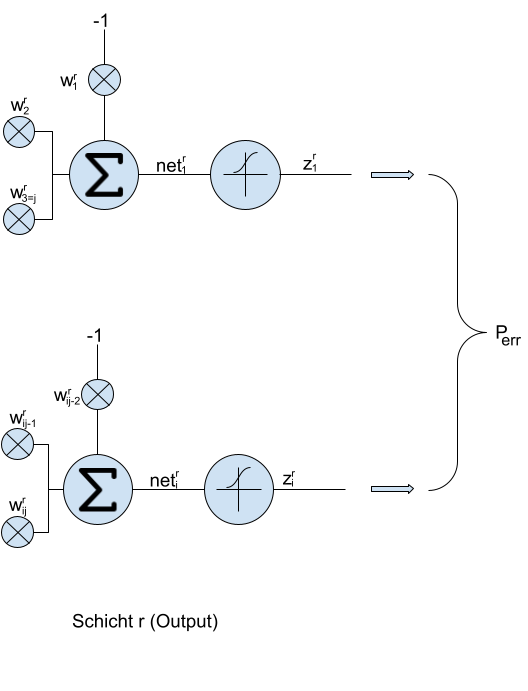
\includegraphics[width=1\linewidth]{../common/01_neuronal_network/00_resources/04_backpropagation_output.png}
    \end{center}
    \caption{Die Output-Schicht eines neuronalen Netzes für Backpropagation}
    \label{fig:08_backpropagation_output}
\end{figure}
Am Ende sollen auch hier die Gewichte korrigiert werden, es wird nun aber ein Zwischenschritt geschaltet.
Dieser Zwischenschritt besteht aus der Berechnung des Terms $\delta_i^r$. Dieser Term beschreibt die Ableitungskette
$\frac{\delta P_{err}}{\delta z_i^r} \cdot \frac{\delta z_i^r}{\delta net_i^r}$. Man beachte, dass es genau so viele Elemente
$\delta_i^r$ wie Neuronen in der Schicht $r$ gibt.
Im Falle des Perceptrons gibt es z.B. nur ein Element, im Falle eines neuronalen Netzes gibt es im Output-Layer so viele Elemente wie
Output-Klassen (Neuronen). Zu diesem Zeitpunkt gibt es noch keine Korrektur der Gewichte.
Es kann also festgehalten werden, dass gilt:
\begin{align}
    \delta_i^r = (d_i^r - z_i^r) \cdot z_i^r(1 - z_i^r) \cdot \label{eq:04_delta_output}
\end{align}

\newpage
Beim zweiten Fall handelt es sich um einen Hidden-Layer. Dazu kann Abbildung \ref{fig:09_backpropagation_hidden} hinzugezogen
werden. Wie vorhin auch steht hier $r$ für die Schicht, welche berechnet werden soll, $i$ für die Anzahl der Neuronen
der Schicht $r$, $j$ für die Anzahl der Gewichte (Inputs) pro Neuron der Schicht $r$, $k$ für die vorher berechnete
Schicht, $l$ für die Anzahl der Neuronen der Schicht $k$, $m$ für die Anzahl der Gewichte pro Neuron der Schicht $k$ (bei einem
Full-Connected Netzwerk gilt $m = i + 1$). Auf der rechten Seite können ebenfalls die bekannten Werte abgelesen werden.
Diese setzen sich aus den bereits vorhin gesehenen Termen\footnote{Anzumerken sei hier, dass es sich bei $l$ nur
um einen Platzhalter handelt. Die Nummerierung geht von $1$ bis $l$, es existieren also $l$ $\delta$.} $\delta_l^k$ zusammen. Es sind die Ableitungen der
Fehlerfunktion $P_{err}$ nach $net_l^k$. Wie bereits erwähnt gibt es so viele Terme, wie Neuronen der Schicht $k$.
\begin{figure}[h!]
    \begin{center}
        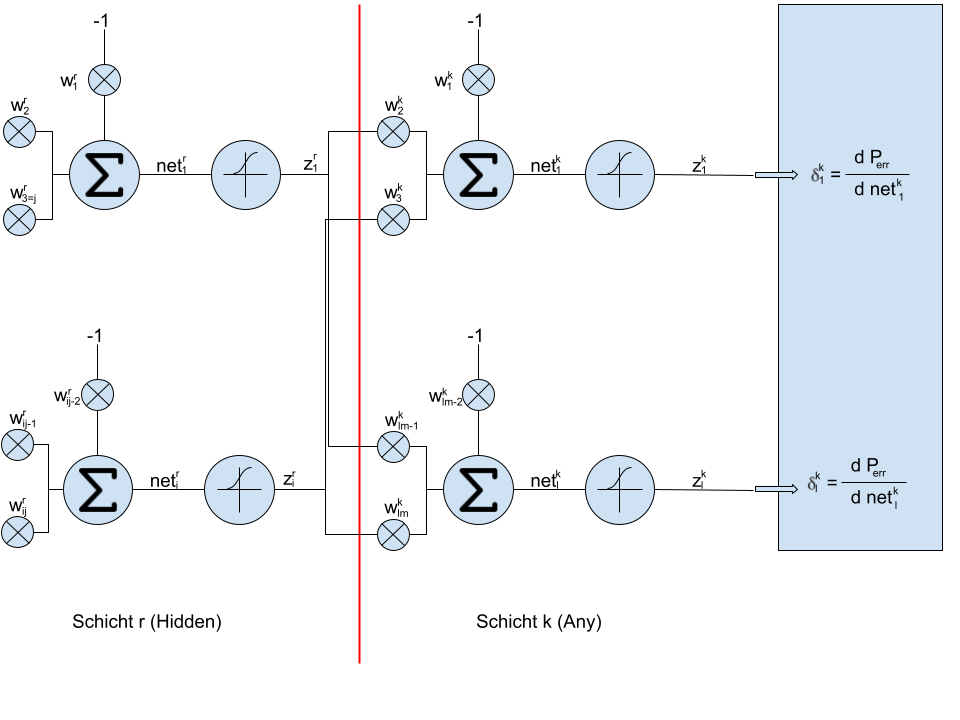
\includegraphics[width=1\linewidth]{../common/01_neuronal_network/00_resources/05_backpropagation_hidden.png}
    \end{center}
    \caption{Zwei Schichten eines neuronalen Netzes für Backpropagation}
    \label{fig:09_backpropagation_hidden}
\end{figure}

Auch in diesem Fall geht es um die Berechnung des Terms $\delta_i^r$ anhand der genannten bekannten Terme. Es müssen wiederum
alle Pfade, welche zu dem Neuron führen, betrachtet werden. Der Term $\delta_i^r$ setzt sich wie nachfolgend zusammen\footnote{Aus der Gleichung \ref{eq:05_delta_hidden} ist ersichtlich, dass es sich bei $nm$ um eine Multiplikation handelt. $n$ läuft
von $1$ bis $l$. Wird $n$ mit der Anzahl Gewichte $m$ pro Neuron der Schicht $k$ multipliziert, wird also jeweils das letzte Gewicht eines
Neurons betrachtet. Dieses führt immer zu $z_i^r$.
}:
\begin{align}
    \delta_1^k = \frac{\delta P_{err}}{\delta net_1^k}\\
    \delta_l^k = \frac{\delta P_{err}}{\delta net_l^k}\\
    \delta_i^r = \frac{\delta z_i^r}{\delta net_i^r} \cdot \delta_1^k \cdot w_3^k + \frac{\delta z_i^r}{\delta net_i^r} \cdot \delta_l^k \cdot w_{lm}^k\\
    \delta_i^r = \frac{\delta z_i^r}{\delta net_i^r} \cdot (\delta_1^k \cdot w_3^k + \delta_l^k \cdot w_{lm}^k)\\
    \delta_i^r = \frac{\delta z_i^r}{\delta net_i^r} \cdot \sum_n^l(\delta_n^k \cdot w_{nm}^k)\\
    \delta_i^r = z_i^r(1 - z_i^r) \cdot \sum_n^l(\delta_n^k \cdot w_{nm}^k)\label{eq:05_delta_hidden}
\end{align}
\\

Da der Term $\delta_i^r$ nun für beide Fälle bekannt ist, können zuletzt die Gewichte korrigiert werden.
Man nehme an, dass es bei den Gewichten der Schicht $r$ die Inputs $x_{ij}^{r-1}$ der vorherigen Schicht $r-1$ gibt,
die ebenso wie die Gewichte nummeriert sind. In dem Fall würde die Korrektur für $w_{ij}^r$ lauten:
\begin{align}
    \delta_i^r = \frac{\delta P_{err}}{\delta net_i^r}\\
    w_{ij, neu}^r = w_{ij, alt}^r + \lambda \cdot \delta_i^r \cdot \frac{net_i^r}{\delta w_{ij}^r}\\
    w_{ij, neu}^r = w_{ij, alt}^r + \lambda \cdot \delta_i^r \cdot x_{ij}^{r-1}
\end{align}

\newpage
Zu guter Letzt kann noch der abschliessende Algorithmus \ref{alg:00_backpropagation} angegeben werden.\\
\begin{algorithm}[H]
    \For{o = last downto 2}{
        \If {o == last}{
            \For{t = 1 to i}{
                $\delta_t^o = (d_t^o - z_t^o) \cdot z_t^o(1 - z_t^o)$
            }
        }
        \Else{
            \For{t = 1 to i}{
                $\delta_t^o = z_t^o(1 - z_t^o) \cdot \sum_n^l(\delta_n^{o + 1} \cdot w_{nm}^{o + 1})$
            }
        }
        \For{(t, h) = (1,1) to (i, j)}{
            $\delta w_{th}^o = \delta_t^o \cdot x_{th}^{o - 1}$\\
            $w_{th, neu}^o = w_{th, alt}^o + \lambda \cdot \delta w_{th}^o$
        }
    }
    \caption{Backpropagation Algorithmus}
    \label{alg:00_backpropagation}
\end{algorithm}
Hierbei gibt $o$ die zu berechnende Schicht an. Diese beginnt am Ende, also beim Output-Layer. Der Input-Layer wird nicht
berücksichtigt, weswegen das Verfahren bei der vorletzten Schicht stoppt.

\newpage
\subsection{XOR und die Lösung}
Um noch ein Beispiel einer nichtlinearen Funktion, welche ein neuronales Netz darstellt, zu nennen, wird das vorherige
Beispiel von \glqq XOR\grqq{} aus Kapitel \ref{chapter:02_xor_perceptron} wiederaufgegriffen. Diesmal wird ein neuronales Netz mit
zwei Inputs, einem Hidden-Layer mit zwei Neuronen sowie einem Output-Layer mit einem Neuron erstellt (siehe Abbildung
\ref{fig:10_xor_neuronal_network}).
\begin{figure}[h!]
    \begin{center}
        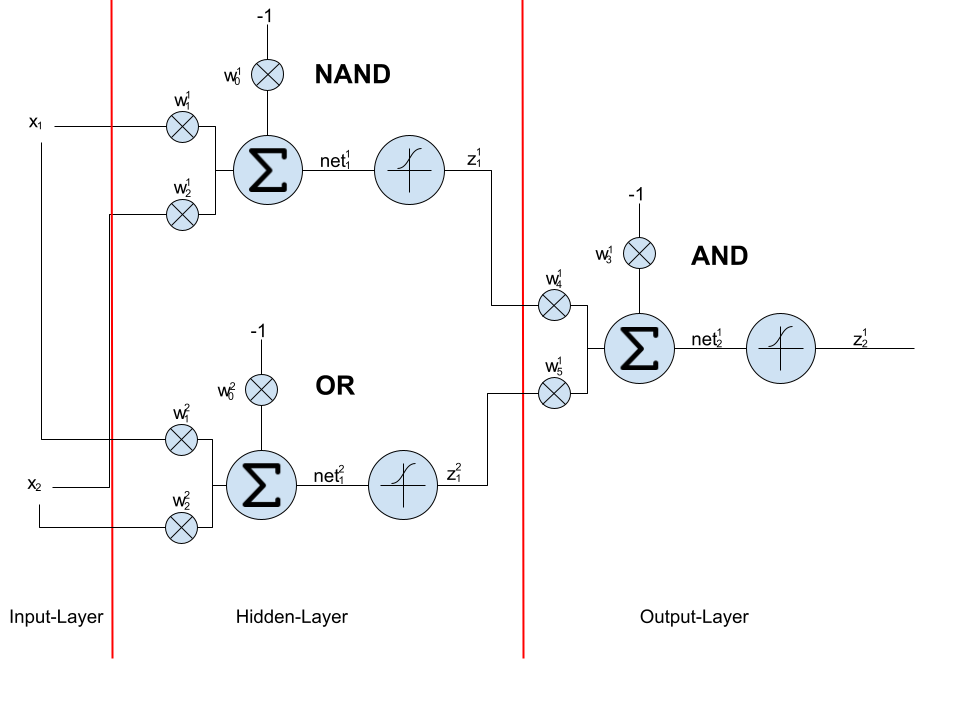
\includegraphics[width=1\linewidth]{../common/01_neuronal_network/00_resources/06_xor_neuronal_network.png}
    \end{center}
    \caption{Ein neuronales Netz für XOR}
    \label{fig:10_xor_neuronal_network}
\end{figure}
\newpage

Hierbei werden die Neuronen der Schichten speziell trainiert. Wie man in der Abbildung \ref{fig:11_xor_neuronal_network_operator}
entnehmen kann, ist \glqq XOR\grqq{} die Kombination durch \glqq AND\grqq{} von \glqq OR\grqq{} und \glqq NAND\grqq{}.
Diese Kombination wird ebenfalls durch das neuronale Netz in Abbildung \ref{fig:10_xor_neuronal_network} erzielt.
\begin{figure}[h!]
    \begin{center}
        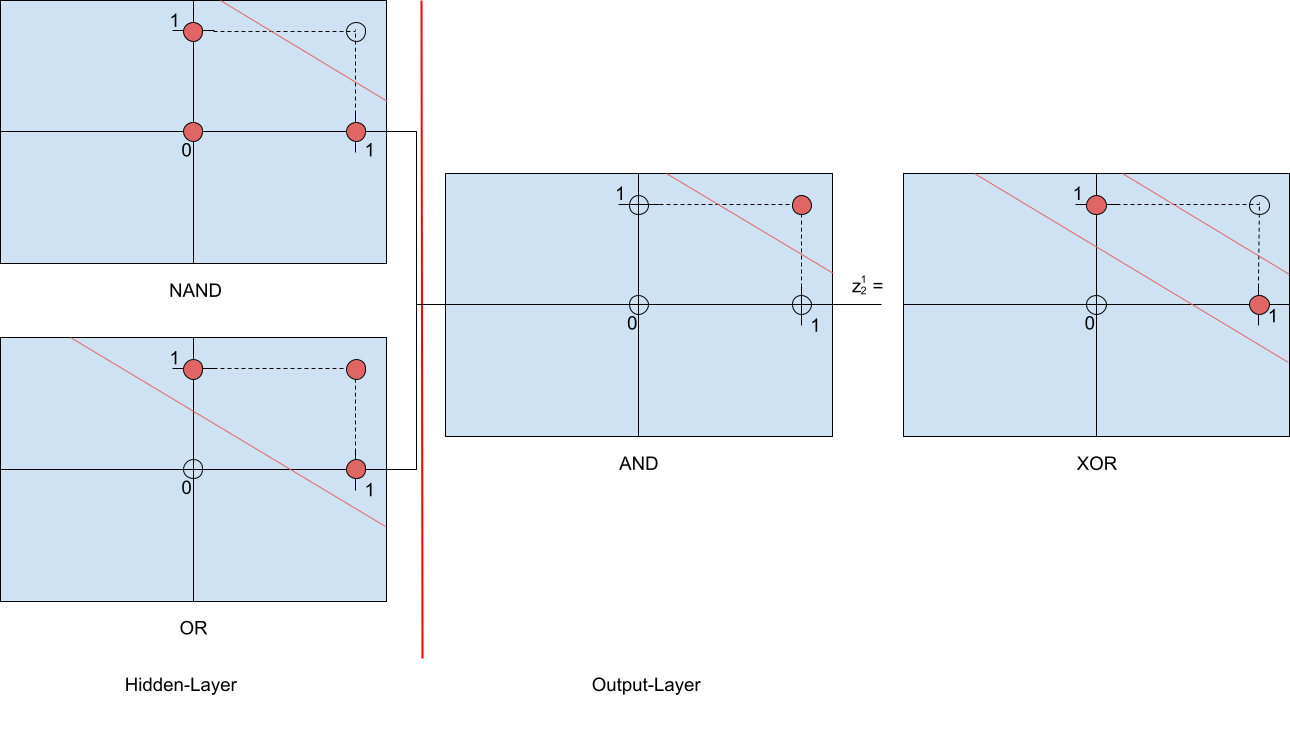
\includegraphics[width=1\linewidth]{../common/01_neuronal_network/00_resources/07_xor_neuronal_network_logical.png}
    \end{center}
    \caption{Die Kombination logischer Operatoren zur Erzielung von XOR}
    \label{fig:11_xor_neuronal_network_operator}
\end{figure}
\\

Mathematisch kann man sich ein \glqq XOR\grqq{} relativ gut vorstellen und dementsprechend die Architektur des neuronalen
Netzes wählen. Bei der Klassifikation in Bilderkennung ist dies jedoch nicht mehr so offensichtlich, weswegen beim Training des
Netzes auch sehr viele verschiedene Architekturen (Anzahl Hidden Layer, Anzahl Neuronen, usw.) ausprobiert werden müssen,
um eine möglichst gute Annäherung zu finden.